
\subsection{Effect of different step sizes for dense SIFT}
\begin{figure}[H]
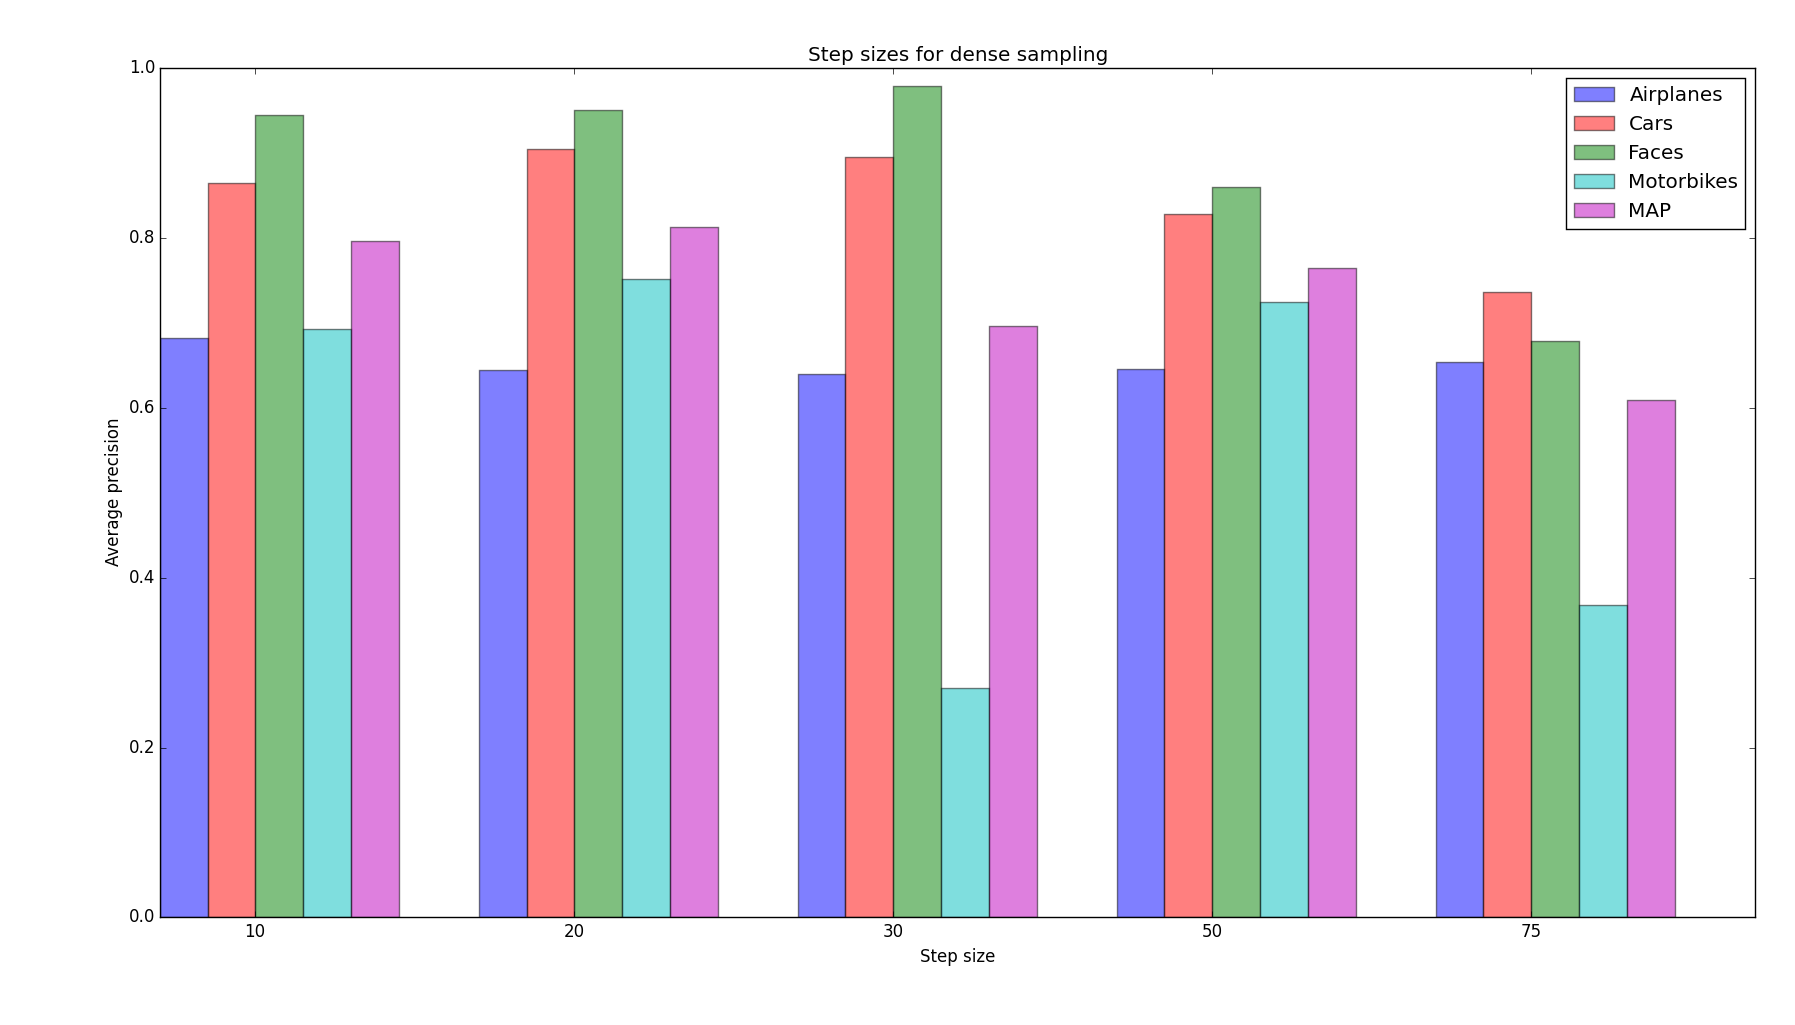
\includegraphics[width=\textwidth]{../plots/step_sizes_dense_sampling}
\caption{Effect of step size on AP}
\label{plot:stepsize}
\end{figure}
\begin{table}[H]
\begin{tabular}{|c|ccccc|}
\hline
\textbf{Step size} & \textbf{AP Airplanes} & \textbf{AP Cars} & \textbf{AP Faces} & \textbf{AP Motorbikes} & \textbf{MAP}\\
\hline
10 & 0.6823 & 0.8654 & 0.9444 & 0.6934 & 0.7964\\
20 & 0.6447 & 0.9053 & 0.9510 & 0.7516 & 0.8132\\
30 & 0.6405 &  0.8952& 0.9792& 0.2704 & 0.6963\\
50 & 0.6463 & 0.8288 & 0.8596 & 0.7247 & 0.7648\\
75 & 0.6539 & 0.7360 & 0.6791 & 0.3673 & 0.6091\\
\hline
\end{tabular}
\caption{Effect of different step sizes for dense SIFT Color space: opponent}
\label{tab:stepsize}
\end{table}

The effect of changing the step sizes for dense SIFT sampling can be see in table \ref{tab:stepsize} and figure \ref{plot:step size}. A small step size, e.g. 10, underperforms compared to a slightly larger step size. However, when the step size is increased even more, the mean average precision of the algorithm rapidly decreases. The tipping point for the step size occurs at 20. This is due to a small step size resulting in a too detail oriented feature extraction, resulting in much noise and a tendency to overfit the data, while a large step size skips many details and tends to underfit the data. 